\documentclass[12pt, twoside]{article}
% \documentclass[12pt, twoside]{article}
\usepackage[letterpaper, margin=1in, headsep=0.2in]{geometry}
\setlength{\headheight}{0.6in}
%\usepackage[english]{babel}
\usepackage[utf8]{inputenc}
\usepackage{microtype}
\usepackage{amsmath}
\usepackage{amssymb}
%\usepackage{amsfonts}
\usepackage[nomessages]{fp} %\FPeval{\var-name}{2*sin(pi/6)}
\usepackage{siunitx} %units in math. eg 20\milli\meter
\usepackage{yhmath} % for arcs, overparenth command
\usepackage{tikz} %graphics
\usetikzlibrary{quotes, angles, arrows, arrows.meta}
\usepackage{graphicx} %consider setting \graphicspath{{images/}}
\usepackage{parskip} %no paragraph indent
\usepackage{enumitem}
\usepackage{multicol}
\usepackage{venndiagram}

\usepackage{fancyhdr}
\pagestyle{fancy}
\fancyhf{}
\renewcommand{\headrulewidth}{0pt} % disable the underline of the header
\raggedbottom
\hfuzz=2mm %suppresses overfull box warnings

\usepackage{hyperref}

\fancyhead[LE]{\thepage}
\fancyhead[RO]{\thepage \\ First and last name: \hspace{2.5cm} \,\\ Section: \hspace{2.5cm} \,}
\fancyhead[LO]{BECA/Huson/Geometry: Construction \\* 8 October 2024}

\begin{document}

%\subsubsection*{2.1 Classwork: Angle measures}
\subsubsection*{1.21 Classwork: Angle measures, transversals}
\begin{enumerate}
\item Use the image of the protractor to measure each of the angles. \par \medskip
  \begin{tikzpicture}
    \draw[thick] (-3,0)--(0,0)--(3,0);
    \draw (4,0) arc (0:180:4);
    \draw[thick] (0,0) circle [radius=0.1];
    \foreach \x in {0,15,30,...,180}
      \node at (\x:3.4){\x};
    \foreach \x in {0,15,30,...,180}
      \draw (\x:3.7)--(\x:4);
    \foreach \x in {0,5,...,180}
      \draw (\x:3.9)--(\x:4);
    \draw[->,thick] (0,0)--(25:4.5)node[right]{m$\angle A = \rule{2cm}{0.1mm}$};
    \draw[->,thick] (0,0)--(68:4.5)node[right]{m$\angle B = \rule{2cm}{0.1mm}$};
    \draw[->,thick] (0,0)--(125:4.5)node[left]{m$\angle C = \rule{2cm}{0.1mm}$};
  \end{tikzpicture}

\item
\begin{enumerate}
  \item Write down the name of the angle below using proper geometric notation.
  \item Find the measure of the angle in degrees with a protractor.
  \item Is it an acute, obtuse, or right angle?
\end{enumerate}
    \begin{flushright}
    \begin{tikzpicture}[scale=2]
      \draw[->, thick] (0,0)--(40:4);
      \draw[->, thick] (0,0)--(-20:5);
      \draw[fill] (40:3) circle [radius=0.025] node[above left ]{$D$};
      \draw[fill] (0,0) circle [radius=0.025] node[above left]{$E$};
      \draw[fill] (-20:4) circle [radius=0.025] node[above]{$F$};
    \end{tikzpicture}
    \end{flushright}

\item Circle True or False for each statement.
\begin{multicols*}{2}
  \begin{enumerate}
    \item T \quad F \quad Point $P$ is the vertex
    \item T \quad F \quad $\overrightarrow{OP}$, $\overrightarrow{OS}$ are opposite rays
    \item T \quad F \quad m$\angle ROS = 90^\circ$
    \item T \quad F \quad $\angle QOS$ is an acute angle
  \end{enumerate}
  \begin{tikzpicture}[scale=0.8, rotate=0]
    \draw[->, thick] (0,0)--(129:4);
    \draw[<->, thick] (-4,0)--(3,0)node[below]{$S$};
    \draw[->, thick] (0,0)--(0,4);
    \draw (0,0)++(0.4,0)--++(0,0.4)--+(-0.4,0);
    \draw[fill] (129:3) circle [radius=0.05] node[below left]{$Q$};
    \draw[fill] (-3,0) circle [radius=0.05] node[below]{$P$}; 
    \draw[fill] (0,0) circle [radius=0.05] node[below]{$O$};
    \draw[fill] (0,3) circle [radius=0.05] node[right]{$R$};
    %\node at (-1,0.4){$51^\circ$};
    %\node at (-0.4,1.2){$x^\circ$};
  \end{tikzpicture}
\end{multicols*}

\newpage
\item Given two parallel lines and a transversal, as shown, with m$\angle 6 =  70^\circ$. Write down the value of each angle measure.
  \begin{multicols}{3}
    \begin{enumerate}[itemsep=0.5cm]
      \item m$\angle 1 = $
      \item m$\angle 2 = $
      \item m$\angle 3 = $
      \item m$\angle 4 = $
      \item m$\angle 5 = $
      \item m$\angle 6 = $
      \item m$\angle 7 = $
      \item m$\angle 8 = $
    \end{enumerate}
      \begin{tikzpicture}[scale=1]
      \draw [<->, thick] (3.5,2)--(7,2);
      \draw [<->, thick] (2.5,0)--(6,0);
      \draw [<->, thick] (4,-1)--(5.5,3);
      \node at (4.5,0.3) [left]{$5$};
      \node at (4.5,0.3) [right]{$6$};
      \node at (4.3,-0.3) [left]{$7$};
      \node at (4.3,-0.3) [right]{$8$};
      \node at (5.2,2) [above left]{$1$};
      \node at (5.2,2) [above right]{$2$};
      \node at (5,2) [below left]{$3$};
      \node at (5,2) [below right]{$4$};
    \end{tikzpicture}
  \end{multicols}

\item Label the relationship of each pair: adjacent, vertical, corresponding, alternate interior, same side interior, alternate exterior, or same side exterior
  \begin{multicols}{2}
    \begin{enumerate}[itemsep=0.5cm]
      \item $\angle 1$,$\angle 4$
      \item $\angle 3$,$\angle 6$
      \item $\angle 5$,$\angle 3$
      \item $\angle 6$,$\angle 2$
      \item $\angle 1$,$\angle 8$
    \end{enumerate}
      \begin{tikzpicture}[scale=1]
      \draw [<->, thick] (3.5,2)--(7,2);
      \draw [<->, thick] (2.5,0)--(6,0);
      \draw [<->, thick] (4,-1)--(5.5,3);
      \node at (4.5,0.3) [left]{$5$};
      \node at (4.5,0.3) [right]{$6$};
      \node at (4.3,-0.3) [left]{$7$};
      \node at (4.3,-0.3) [right]{$8$};
      \node at (5.2,2) [above left]{$1$};
      \node at (5.2,2) [above right]{$2$};
      \node at (5,2) [below left]{$3$};
      \node at (5,2) [below right]{$4$};
    \end{tikzpicture}
  \end{multicols}

\item Identify each angle
  \begin{multicols}{2}
  \begin{enumerate}
    \item Opposite $\angle 4$
    \item Corresponding to $\angle 3$
    \item Alternate exterior to $\angle 8$
    \item Same side interior to $\angle 5$
    \item Alternate interior to $\angle 4$
  \end{enumerate}
  \begin{center}
  \begin{tikzpicture}[scale=1.2]
    \draw [<->, thick] (3,2)--(7,2);
    \draw [<->, thick] (2,0)--(6,0);
    \draw [<->, thick] (4,-1)--(5.5,3);
    \node at (4.5,0.3) [left]{$5$};
    \node at (4.5,0.3) [right]{$6$};
    \node at (4.3,-0.3) [left]{$7$};
    \node at (4.3,-0.3) [right]{$8$};
    \node at (5.2,2) [above left]{$1$};
    \node at (5.2,2) [above right]{$2$};
    \node at (5,2) [below left]{$3$};
    \node at (5,2) [below right]{$4$};
  \end{tikzpicture}
  \end{center}
  \end{multicols}
  
\newpage
\item Using the given ray $\overrightarrow{AB}$ as one leg, draw an angle that measures $55^\circ$. \par \vspace{5cm} \hspace{3cm}
  \tikz{
    \draw[->, thick] (0,0)--(0:8)node[below left]{$B$};
    \fill (0,0) circle [radius=0.07cm]node[below]{$A$};}

\item Draw the square $ABCD$ having the base $\overline{AB}$. (use a straight edge and protracter or square to work accurately)
\begin{enumerate}
  \item Label the vertices $C$, $D$ and mark the side congruencies with hash marks. Measure and mark the length in centimeters of $\overline{AB}$. (label the units)
  \item Draw the diagonal $\overline{AC}$ with a dashed line. Measure and label its length rounded to the \emph{nearest tenth of a centimeter} (nearest millimeter).
\end{enumerate}
\vspace{5cm}
\begin{center}
  \tikz{
  \draw[thick] (0,0)--(5,0);
  \fill (0,0) circle [radius=0.07cm]node[below]{$A$};
  \fill (5,0) circle [radius=0.07cm]node[below]{$B$};}
\end{center}

\item Write the appropriate name for the type of angle depending on its measure in degrees. (acute, right, obtuse, or straight) \bigskip
  \begin{enumerate}
    \item m$\angle = 90$ : \rule{4cm}{0.15mm} \bigskip
    \item $90 < \text{m}\angle < 180$ : \rule{4cm}{0.15mm} \bigskip
    \item $0< \text{m}\angle < 90$ : \rule{4cm}{0.15mm} \bigskip
    \item m$\angle = 180$ : \rule{4cm}{0.15mm} \bigskip
  \end{enumerate}


\end{enumerate}
\end{document}